% Created by tikzDevice version 0.12 on 2019-04-13 14:06:17
% !TEX encoding = UTF-8 Unicode
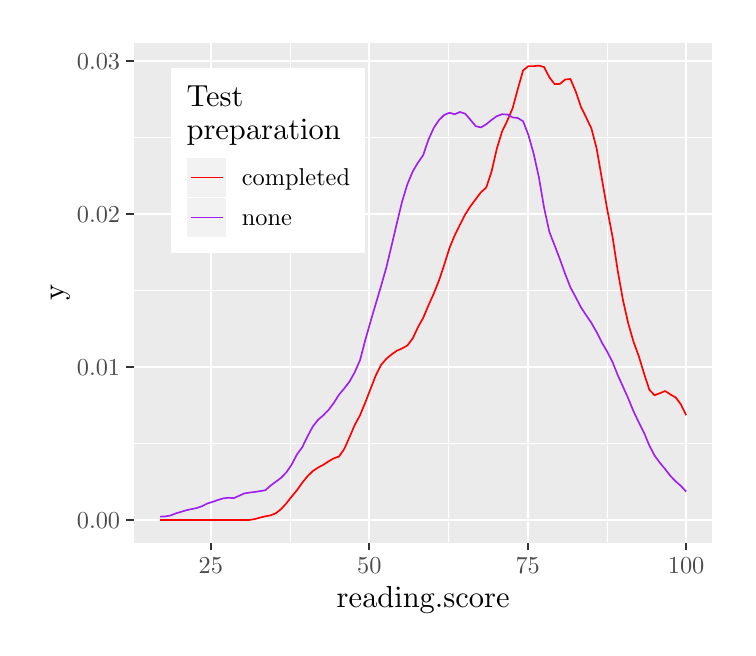
\begin{tikzpicture}[x=1pt,y=1pt]
\definecolor{fillColor}{RGB}{255,255,255}
\path[use as bounding box,fill=fillColor,fill opacity=0.00] (0,0) rectangle (252.94,216.81);
\begin{scope}
\path[clip] (  0.00,  0.00) rectangle (252.94,216.81);
\definecolor{drawColor}{RGB}{255,255,255}
\definecolor{fillColor}{RGB}{255,255,255}

\path[draw=drawColor,line width= 0.6pt,line join=round,line cap=round,fill=fillColor] (  0.00,  0.00) rectangle (252.94,216.81);
\end{scope}
\begin{scope}
\path[clip] ( 38.36, 30.72) rectangle (247.44,211.31);
\definecolor{fillColor}{gray}{0.92}

\path[fill=fillColor] ( 38.36, 30.72) rectangle (247.44,211.31);
\definecolor{drawColor}{RGB}{255,255,255}

\path[draw=drawColor,line width= 0.3pt,line join=round] ( 38.36, 66.55) --
	(247.44, 66.55);

\path[draw=drawColor,line width= 0.3pt,line join=round] ( 38.36,121.79) --
	(247.44,121.79);

\path[draw=drawColor,line width= 0.3pt,line join=round] ( 38.36,177.03) --
	(247.44,177.03);

\path[draw=drawColor,line width= 0.3pt,line join=round] ( 94.81, 30.72) --
	( 94.81,211.31);

\path[draw=drawColor,line width= 0.3pt,line join=round] (152.06, 30.72) --
	(152.06,211.31);

\path[draw=drawColor,line width= 0.3pt,line join=round] (209.32, 30.72) --
	(209.32,211.31);

\path[draw=drawColor,line width= 0.6pt,line join=round] ( 38.36, 38.93) --
	(247.44, 38.93);

\path[draw=drawColor,line width= 0.6pt,line join=round] ( 38.36, 94.17) --
	(247.44, 94.17);

\path[draw=drawColor,line width= 0.6pt,line join=round] ( 38.36,149.41) --
	(247.44,149.41);

\path[draw=drawColor,line width= 0.6pt,line join=round] ( 38.36,204.65) --
	(247.44,204.65);

\path[draw=drawColor,line width= 0.6pt,line join=round] ( 66.19, 30.72) --
	( 66.19,211.31);

\path[draw=drawColor,line width= 0.6pt,line join=round] (123.44, 30.72) --
	(123.44,211.31);

\path[draw=drawColor,line width= 0.6pt,line join=round] (180.69, 30.72) --
	(180.69,211.31);

\path[draw=drawColor,line width= 0.6pt,line join=round] (237.94, 30.72) --
	(237.94,211.31);
\definecolor{drawColor}{RGB}{255,0,0}

\path[draw=drawColor,line width= 0.6pt,line join=round] ( 47.86, 38.93) --
	( 49.77, 38.93) --
	( 51.67, 38.93) --
	( 53.57, 38.93) --
	( 55.47, 38.93) --
	( 57.37, 38.93) --
	( 59.27, 38.93) --
	( 61.17, 38.93) --
	( 63.07, 38.93) --
	( 64.97, 38.93) --
	( 66.87, 38.93) --
	( 68.77, 38.93) --
	( 70.67, 38.93) --
	( 72.57, 38.93) --
	( 74.48, 38.93) --
	( 76.38, 38.93) --
	( 78.28, 38.93) --
	( 80.18, 38.93) --
	( 82.08, 39.24) --
	( 83.98, 39.78) --
	( 85.88, 40.23) --
	( 87.78, 40.58) --
	( 89.68, 41.36) --
	( 91.58, 42.85) --
	( 93.48, 44.96) --
	( 95.38, 47.35) --
	( 97.28, 49.64) --
	( 99.19, 52.34) --
	(101.09, 54.68) --
	(102.99, 56.54) --
	(104.89, 57.83) --
	(106.79, 58.84) --
	(108.69, 60.07) --
	(110.59, 61.17) --
	(112.49, 61.82) --
	(114.39, 64.56) --
	(116.29, 68.83) --
	(118.19, 73.25) --
	(120.09, 76.74) --
	(121.99, 81.35) --
	(123.90, 86.28) --
	(125.80, 91.16) --
	(127.70, 94.95) --
	(129.60, 97.16) --
	(131.50, 98.73) --
	(133.40,100.08) --
	(135.30,100.91) --
	(137.20,101.96) --
	(139.10,104.46) --
	(141.00,108.51) --
	(142.90,111.91) --
	(144.80,116.39) --
	(146.70,120.64) --
	(148.61,125.42) --
	(150.51,131.12) --
	(152.41,137.13) --
	(154.31,141.77) --
	(156.21,145.63) --
	(158.11,149.34) --
	(160.01,152.30) --
	(161.91,154.83) --
	(163.81,157.36) --
	(165.71,159.04) --
	(167.61,164.77) --
	(169.51,173.03) --
	(171.41,179.25) --
	(173.32,183.21) --
	(175.22,187.63) --
	(177.12,194.70) --
	(179.02,201.36) --
	(180.92,202.90) --
	(182.82,202.90) --
	(184.72,203.10) --
	(186.62,202.57) --
	(188.52,198.86) --
	(190.42,196.40) --
	(192.32,196.49) --
	(194.22,198.07) --
	(196.12,198.27) --
	(198.03,193.75) --
	(199.93,188.19) --
	(201.83,184.33) --
	(203.73,180.32) --
	(205.63,172.98) --
	(207.53,161.94) --
	(209.43,151.09) --
	(211.33,141.31) --
	(213.23,128.88) --
	(215.13,118.26) --
	(217.03,109.89) --
	(218.93,103.28) --
	(220.83, 98.09) --
	(222.74, 91.78) --
	(224.64, 85.98) --
	(226.54, 83.97) --
	(228.44, 84.73) --
	(230.34, 85.52) --
	(232.24, 84.26) --
	(234.14, 83.21) --
	(236.04, 80.68) --
	(237.94, 76.77);
\definecolor{drawColor}{RGB}{160,32,240}

\path[draw=drawColor,line width= 0.6pt,line join=round] ( 47.86, 40.12) --
	( 49.77, 40.21) --
	( 51.67, 40.54) --
	( 53.57, 41.31) --
	( 55.47, 41.87) --
	( 57.37, 42.45) --
	( 59.27, 42.85) --
	( 61.17, 43.26) --
	( 63.07, 43.93) --
	( 64.97, 44.89) --
	( 66.87, 45.47) --
	( 68.77, 46.15) --
	( 70.67, 46.73) --
	( 72.57, 46.94) --
	( 74.48, 46.81) --
	( 76.38, 47.64) --
	( 78.28, 48.52) --
	( 80.18, 48.81) --
	( 82.08, 49.04) --
	( 83.98, 49.35) --
	( 85.88, 49.66) --
	( 87.78, 51.35) --
	( 89.68, 52.75) --
	( 91.58, 54.15) --
	( 93.48, 56.11) --
	( 95.38, 58.92) --
	( 97.28, 62.57) --
	( 99.19, 65.15) --
	(101.09, 69.07) --
	(102.99, 72.61) --
	(104.89, 75.07) --
	(106.79, 76.71) --
	(108.69, 78.63) --
	(110.59, 81.16) --
	(112.49, 84.18) --
	(114.39, 86.43) --
	(116.29, 88.91) --
	(118.19, 92.32) --
	(120.09, 96.65) --
	(121.99,103.93) --
	(123.90,110.64) --
	(125.80,117.09) --
	(127.70,123.48) --
	(129.60,130.16) --
	(131.50,138.06) --
	(133.40,146.15) --
	(135.30,153.97) --
	(137.20,160.22) --
	(139.10,164.77) --
	(141.00,167.99) --
	(142.90,170.72) --
	(144.80,176.28) --
	(146.70,180.50) --
	(148.61,183.41) --
	(150.51,185.27) --
	(152.41,186.05) --
	(154.31,185.52) --
	(156.21,186.35) --
	(158.11,185.71) --
	(160.01,183.50) --
	(161.91,181.20) --
	(163.81,180.76) --
	(165.71,181.91) --
	(167.61,183.47) --
	(169.51,184.82) --
	(171.41,185.52) --
	(173.32,185.42) --
	(175.22,184.39) --
	(177.12,184.16) --
	(179.02,182.99) --
	(180.92,178.08) --
	(182.82,171.35) --
	(184.72,162.79) --
	(186.62,151.66) --
	(188.52,142.99) --
	(190.42,138.11) --
	(192.32,133.14) --
	(194.22,127.82) --
	(196.12,122.96) --
	(198.03,119.44) --
	(199.93,115.72) --
	(201.83,112.86) --
	(203.73,110.07) --
	(205.63,106.73) --
	(207.53,102.94) --
	(209.43, 99.70) --
	(211.33, 95.99) --
	(213.23, 91.23) --
	(215.13, 87.05) --
	(217.03, 82.80) --
	(218.93, 78.15) --
	(220.83, 74.15) --
	(222.74, 70.40) --
	(224.64, 65.83) --
	(226.54, 62.18) --
	(228.44, 59.59) --
	(230.34, 57.32) --
	(232.24, 54.84) --
	(234.14, 52.89) --
	(236.04, 51.22) --
	(237.94, 49.18);
\end{scope}
\begin{scope}
\path[clip] (  0.00,  0.00) rectangle (252.94,216.81);
\definecolor{drawColor}{gray}{0.30}

\node[text=drawColor,anchor=base east,inner sep=0pt, outer sep=0pt, scale=  0.88] at ( 33.41, 35.90) {0.00};

\node[text=drawColor,anchor=base east,inner sep=0pt, outer sep=0pt, scale=  0.88] at ( 33.41, 91.14) {0.01};

\node[text=drawColor,anchor=base east,inner sep=0pt, outer sep=0pt, scale=  0.88] at ( 33.41,146.38) {0.02};

\node[text=drawColor,anchor=base east,inner sep=0pt, outer sep=0pt, scale=  0.88] at ( 33.41,201.62) {0.03};
\end{scope}
\begin{scope}
\path[clip] (  0.00,  0.00) rectangle (252.94,216.81);
\definecolor{drawColor}{gray}{0.20}

\path[draw=drawColor,line width= 0.6pt,line join=round] ( 35.61, 38.93) --
	( 38.36, 38.93);

\path[draw=drawColor,line width= 0.6pt,line join=round] ( 35.61, 94.17) --
	( 38.36, 94.17);

\path[draw=drawColor,line width= 0.6pt,line join=round] ( 35.61,149.41) --
	( 38.36,149.41);

\path[draw=drawColor,line width= 0.6pt,line join=round] ( 35.61,204.65) --
	( 38.36,204.65);
\end{scope}
\begin{scope}
\path[clip] (  0.00,  0.00) rectangle (252.94,216.81);
\definecolor{drawColor}{gray}{0.20}

\path[draw=drawColor,line width= 0.6pt,line join=round] ( 66.19, 27.97) --
	( 66.19, 30.72);

\path[draw=drawColor,line width= 0.6pt,line join=round] (123.44, 27.97) --
	(123.44, 30.72);

\path[draw=drawColor,line width= 0.6pt,line join=round] (180.69, 27.97) --
	(180.69, 30.72);

\path[draw=drawColor,line width= 0.6pt,line join=round] (237.94, 27.97) --
	(237.94, 30.72);
\end{scope}
\begin{scope}
\path[clip] (  0.00,  0.00) rectangle (252.94,216.81);
\definecolor{drawColor}{gray}{0.30}

\node[text=drawColor,anchor=base,inner sep=0pt, outer sep=0pt, scale=  0.88] at ( 66.19, 19.71) {25};

\node[text=drawColor,anchor=base,inner sep=0pt, outer sep=0pt, scale=  0.88] at (123.44, 19.71) {50};

\node[text=drawColor,anchor=base,inner sep=0pt, outer sep=0pt, scale=  0.88] at (180.69, 19.71) {75};

\node[text=drawColor,anchor=base,inner sep=0pt, outer sep=0pt, scale=  0.88] at (237.94, 19.71) {100};
\end{scope}
\begin{scope}
\path[clip] (  0.00,  0.00) rectangle (252.94,216.81);
\definecolor{drawColor}{RGB}{0,0,0}

\node[text=drawColor,anchor=base,inner sep=0pt, outer sep=0pt, scale=  1.10] at (142.90,  7.44) {reading.score};
\end{scope}
\begin{scope}
\path[clip] (  0.00,  0.00) rectangle (252.94,216.81);
\definecolor{drawColor}{RGB}{0,0,0}

\node[text=drawColor,rotate= 90.00,anchor=base,inner sep=0pt, outer sep=0pt, scale=  1.10] at ( 13.08,121.02) {y};
\end{scope}
\begin{scope}
\path[clip] (  0.00,  0.00) rectangle (252.94,216.81);
\definecolor{fillColor}{RGB}{255,255,255}

\path[fill=fillColor] ( 51.94,135.47) rectangle (121.99,202.28);
\end{scope}
\begin{scope}
\path[clip] (  0.00,  0.00) rectangle (252.94,216.81);
\definecolor{drawColor}{RGB}{0,0,0}

\node[text=drawColor,anchor=base west,inner sep=0pt, outer sep=0pt, scale=  1.10] at ( 57.44,188.23) {Test };

\node[text=drawColor,anchor=base west,inner sep=0pt, outer sep=0pt, scale=  1.10] at ( 57.44,176.35) { preparation};
\end{scope}
\begin{scope}
\path[clip] (  0.00,  0.00) rectangle (252.94,216.81);
\definecolor{drawColor}{RGB}{255,255,255}
\definecolor{fillColor}{gray}{0.95}

\path[draw=drawColor,line width= 0.6pt,line join=round,line cap=round,fill=fillColor] ( 57.44,155.43) rectangle ( 71.89,169.88);
\end{scope}
\begin{scope}
\path[clip] (  0.00,  0.00) rectangle (252.94,216.81);
\definecolor{drawColor}{RGB}{255,0,0}

\path[draw=drawColor,line width= 0.6pt,line join=round] ( 58.88,162.65) -- ( 70.45,162.65);
\end{scope}
\begin{scope}
\path[clip] (  0.00,  0.00) rectangle (252.94,216.81);
\definecolor{drawColor}{RGB}{255,0,0}

\path[draw=drawColor,line width= 0.6pt,line join=round] ( 58.88,162.65) -- ( 70.45,162.65);
\end{scope}
\begin{scope}
\path[clip] (  0.00,  0.00) rectangle (252.94,216.81);
\definecolor{drawColor}{RGB}{255,255,255}
\definecolor{fillColor}{gray}{0.95}

\path[draw=drawColor,line width= 0.6pt,line join=round,line cap=round,fill=fillColor] ( 57.44,140.97) rectangle ( 71.89,155.43);
\end{scope}
\begin{scope}
\path[clip] (  0.00,  0.00) rectangle (252.94,216.81);
\definecolor{drawColor}{RGB}{160,32,240}

\path[draw=drawColor,line width= 0.6pt,line join=round] ( 58.88,148.20) -- ( 70.45,148.20);
\end{scope}
\begin{scope}
\path[clip] (  0.00,  0.00) rectangle (252.94,216.81);
\definecolor{drawColor}{RGB}{160,32,240}

\path[draw=drawColor,line width= 0.6pt,line join=round] ( 58.88,148.20) -- ( 70.45,148.20);
\end{scope}
\begin{scope}
\path[clip] (  0.00,  0.00) rectangle (252.94,216.81);
\definecolor{drawColor}{RGB}{0,0,0}

\node[text=drawColor,anchor=base west,inner sep=0pt, outer sep=0pt, scale=  0.88] at ( 77.39,159.62) {completed};
\end{scope}
\begin{scope}
\path[clip] (  0.00,  0.00) rectangle (252.94,216.81);
\definecolor{drawColor}{RGB}{0,0,0}

\node[text=drawColor,anchor=base west,inner sep=0pt, outer sep=0pt, scale=  0.88] at ( 77.39,145.17) {none};
\end{scope}
\end{tikzpicture}
